\section {API REST base}

    \par Esta seção do presente TCC tem como objetivo apresentar a API REST escolhida para a refatoração, bem como documentar o processo de sua criação, desde a configuração de um ambiente de desenvolvimento utilizando a ferramenta Docker até a descrição das etapas necessárias para a implementação da API REST. Dessa forma, busca-se fornecer uma base prática para a aplicação da Arquitetura Limpa, contribuindo para uma melhor compreensão dos princípios abordados neste trabalho.
    
    \par A API escolhida como base para este TCC foi uma API REST desenvolvida em um tutorial do Programa de Educação Tutorial (PET) do curso de Sistemas de Informação da UFSM. O material foi disponibilizado pelo Grupo PET no endereço eletrônico\footnote{Disponível em: \url{https://www.ufsm.br/pet/sistemas-de-informacao/2020/08/25/api-laravel}. Acesso em: 25 de novembro de 2025}. O tutorial foi publicado em 25/08/2020 e atualizado em 02/09/2025, permanecendo disponível até a elaboração deste trabalho.

    \par A API desenvolvida no tutorial do PET, consiste em rotas para a gestão do recurso de contatos, de maneira que seja fácil exemplificar o uso das ferramentas do \textit{framework}. Ela foi construída passo a passo, desde a criação do projeto até a implementação de métodos como index, show, store, update e destroy, permitindo uma compreensão clara e objetiva do processo de desenvolvimento de APIs com Laravel.
    
    \par A escolha desse projeto de API REST como base, deve-se à sua clareza e à sua aderência ao padrão de arquitetura MVC, bem como aos padrões nativos do \textit{framework} Laravel. Portanto, a criação da API base seguiu as diretrizes do tutorial, mantendo a estrutura e o fluxo de dados tradicionais do Laravel. Esta etapa inicial não incluiu a implementação de princípios da Arquitetura Limpa, servindo, portanto, como uma referência e um ponto de partida para a refatoração. O objetivo principal foi ter um projeto funcional e representativo do padrão MVC, que é o objeto de estudo e de transformação ao longo deste TCC.

    \subsection{Instalação do Laravel}
    
        \par Para criar a API REST proposta no tutorial do PET, foi usado o sistema operacional Ubuntu 22.04.5 LTS, com as seguintes ferramentas instaladas:

        \begin{itemize}
            \item \textbf{PHP 8.4.1} – Necessário para executar o Composer e criar o projeto Laravel.
            \item \textbf{Composer} – Usado para gerenciador de dependências PHP e instalar o Laravel e seus pacotes.
            \item \textbf{Git} - Para controle de versão do projeto.
            \item \textbf{Docker} - para criar contêineres isolados para a aplicação, servidor web e banco de dados.
            \item \textbf{Docker Compose} - para orquestrar múltiplos \textit{containers} com um único arquivo de configuração.
        \end{itemize}

        \par Considerando as ferramentas citadas anteriormente, foi criado um repositório no GitHub para disponibilizar o código-fonte do projeto de forma completa e replicável, acessível na seguinte URL: \url{https://github.com/williamtrindade/clean-architecture-laravel-api}.

        \par O primeiro passo foi clonar o repositório vazio do GitHub criado e instalar o projeto Laravel utilizando a ferramenta de linha de comando do PHP, o Composer. Inicialmente, foi criado o projeto em uma pasta temporária chamada \texttt{temp} com o comando:
        \begin{verbatim}
        composer create-project laravel/laravel temp
        \end{verbatim}
    
        \par Em seguida, todos os arquivos do projeto foram movidos da pasta \texttt{temp} para a raiz do diretório atual, incluindo arquivos ocultos, e quaisquer mensagens de erro foram redirecionadas para \texttt{/dev/null}:
        \begin{verbatim}
        mv temp/* temp/.* . 2>/dev/null
        \end{verbatim}
        Após a movimentação dos arquivos, a pasta temporária \texttt{temp} foi removida com o comando:
        \begin{verbatim}
        rm -rf temp
        \end{verbatim}

    \subsection{Docker}

        \par Para garantir um ambiente de desenvolvimento isolado, consistente e portátil para replicação do projeto, foi utilizada a tecnologia Docker. O uso de \textit{containers} Docker permitiu encapsular a aplicação e suas dependências, como o servidor web e o banco de dados, eliminando problemas de compatibilidade entre diferentes sistemas operacionais, a orquestração dos serviços foi realizada com o Docker Compose.
        
        \par Conforme a Figura \ref{fig:figura_tutorial_1}, a estrutura de diretórios do projeto foi organizada para acomodar os arquivos de configuração do Docker junto ao projeto Laravel na raiz do mesmo. No diretório reservado ao docker \texttt{/docker}, contém a pasta \texttt{app} que armazena o Dockerfile do projeto e a pasta \texttt{nginx} que armazena a configuração do servidor web Nginx, que atua como ponto de entrada para as requisições HTTP.

        \par Ainda na Figura \ref{fig:figura_tutorial_1} pode-se notar o arquivo \texttt{docker-compose.yml} que é o componente central para a orquestração dos serviços, definindo o uso de \textit{containers} para a aplicação, servidor web e banco de dados.

        \begin{figure}[H]
            \centering
            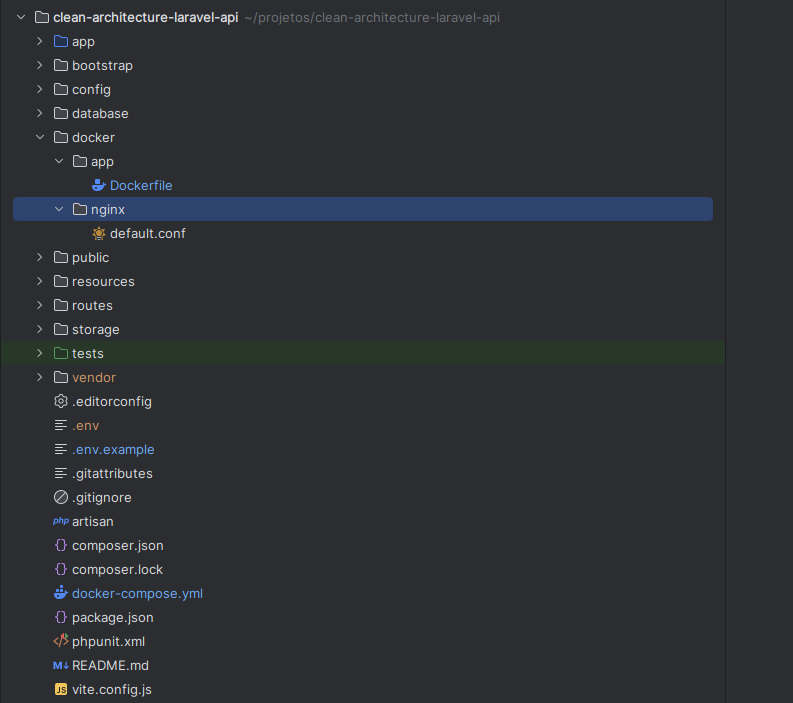
\includegraphics[width=0.9\textwidth]{figuras/tutorial/1estrutura.png}
            \caption{Estrutura de pastas do projeto}
            \label{fig:figura_tutorial_1}
            \newcommand{\minhafonteum}{Fonte: Autor}
            \minhafonteum
        \end{figure}

        \par O Dockerfile é o primeiro componente criado para o ambiente Docker, atuando como um ``manual de instruções'' para a construção da imagem do \textit{container} da aplicação. Ele utiliza a imagem base \texttt{php:8.2-fpm-alpine}, garantindo um ambiente leve e focado no processamento de scripts PHP. 

        \par Através de comandos RUN, o arquivo instala dependências essenciais, como o Git e bibliotecas de desenvolvimento, além de extensões PHP específicas, como a \texttt{pdo\_mysql}, que é necessária para a comunicação com o banco de dados. Por fim, o Dockerfile instala o Composer para gerenciar as dependências do Laravel e define o diretório de trabalho, garantindo que o contêiner esteja pronto para executar a aplicação. O Código \ref{lst:dockerfile} apresenta o código escrito no Dockerfile.

        \lstinputlisting[
            language=bash,
            inputencoding=utf8,
            caption={Código do Dockerfile.},
            label=lst:dockerfile,
            frame=single, % Adiciona uma moldura ao redor do código
            numbers=left, % Adiciona números de linha à esquerda
            breaklines=true, % Quebra linhas longas automaticamente
            basicstyle=\ttfamily\scriptsize % Define a fonte como monoespaçada e pequena
        ]{codigos/ca/docker/app/Dockerfile}

        \par O arquivo \texttt{default.conf}, localizado na pasta \texttt{docker/nginx}, é o responsável por configurar o servidor web Nginx. Sua principal função é atuar como um proxy reverso, recebendo todas as requisições HTTP e encaminhando-as para o \textit{container} da aplicação PHP.

        \par Dentro deste arquivo, a diretiva \texttt{root} é configurada para apontar para a pasta public do Laravel, que é o ponto de entrada da aplicação. A regra de \texttt{location /} garante que todas as requisições para URLs que não correspondem a arquivos existentes sejam redirecionadas para o \texttt{index.php} do Laravel, o que é fundamental para o sistema de roteamento do \textit{framework}.

        \par A seção \texttt{location \textasciitilde \textbackslash.php\$} é a mais crítica para o funcionamento da aplicação. Ela intercepta todas as requisições que terminam em .php e as encaminha para o serviço app (o \textit{container} PHP-FPM) na porta 9000. Essa configuração permite que o Nginx entregue arquivos estáticos diretamente e passe apenas as requisições dinâmicas para o PHP processar, otimizando o desempenho.

        \par No Código \ref{defaultconf} é apresentada a estrutura do arquivo \texttt{default.conf}.

        \lstinputlisting[
            language=bash,
            inputencoding=utf8,
            caption={Código do default.conf.},
            label=defaultconf,
            frame=single, % Adiciona uma moldura ao redor do código
            numbers=left, % Adiciona números de linha à esquerda
            breaklines=true, % Quebra linhas longas automaticamente
            basicstyle=\ttfamily\scriptsize % Define a fonte como monoespaçada e pequena
        ]{codigos/ca/docker/nginx/default.conf}

        \par O arquivo \texttt{docker-compose.yml} é o componente central para a orquestração do ambiente, atuando como um plano que define e gerencia os serviços da aplicação. Ele garante que cada serviço, como a aplicação Laravel, o servidor Nginx e o banco de dados MySQL, sejam criados e interligados corretamente, eliminando a complexidade de iniciar cada contêiner de maneira individual.

        \par Este arquivo é dividido em três seções principais:

        \begin{enumerate}
            \item \textbf{services}: Esta seção define os \textit{containers} que compõem a aplicação.
            \begin{itemize}
                \item \textbf{\texttt{app}}: Este serviço constrói o \textit{container} da aplicação, utilizando o \texttt{Dockerfile}. A diretiva \texttt{volumes} serve para que o código do projeto na máquina host seja sincronizado com o código dentro do \textit{container}.
                
                \item \textbf{\texttt{nginx}}: O \textit{container} do Nginx atua como um servidor web e \textit{proxy reverso}. Ele mapeia a porta \texttt{8000} da máquina host para a porta \texttt{80} do \textit{container}, permitindo que o acesso à aplicação pelo navegador.
                
                \item \textbf{\texttt{db}}: Este serviço cria o contêiner do MySQL. A diretiva \texttt{environment} configura o banco de dados com variáveis definidas no arquivo \texttt{.env}, enquanto a diretiva \texttt{volumes} garante a persistência dos dados. O mapeamento da porta \texttt{3307:3306} permite que o \textit{container} do banco de dados seja acessado na porta \texttt{3307} da máquina host, evitando conflitos com outras instalações do MySQL.
            \end{itemize}
        
            \item \textbf{networks}: Define uma rede virtual (\texttt{laravel-network}) que faz com que todos os serviços se comuniquem entre si de forma segura, usando seus nomes de serviço (\texttt{app}, \texttt{nginx}, \texttt{db}) como endereços.
        
            \item \textbf{volumes}: Gerencia a persistência dos dados do banco de dados, para que os dados não sejam perdidos quando o contêiner for parado ou recriado.
        \end{enumerate}
    
        \par No Código \ref{lst:figura.tutorial.4} é apresentado o conteúdo do arquivo \texttt{docker-compose.yml}.

        \lstinputlisting[
            language=bash,
            inputencoding=utf8,
            caption={Código do docker-compose.yml},
            label=lst:figura.tutorial.4,
            frame=single, % Adiciona uma moldura ao redor do código
            numbers=left, % Adiciona números de linha à esquerda
            breaklines=true, % Quebra linhas longas automaticamente
            basicstyle=\ttfamily\scriptsize % Define a fonte como monoespaçada e pequena
        ]{codigos/ca/docker-compose.yml}
        
    
        \par Após a configuração do ambiente Docker, o próximo passo foi preparar o ambiente de desenvolvimento da aplicação. Para isso, o arquivo \texttt{.env.example}, que contém um modelo das variáveis de ambiente padrão do projeto, precisou ser copiado e renomeado para \texttt{.env}. Esse arquivo é fundamental, pois armazena credenciais e configurações sensíveis, como chaves de acesso e informações de conexão com o banco de dados.

        \begin{sloppypar}
            \par É no arquivo .env que as variáveis como \texttt{DB\_CONNECTION}, \texttt{DB\_HOST}, \texttt{DB\_PORT},  \texttt{DB\_DATABASE}, \texttt{DB\_USERNAME}, \texttt{DB\_PASSWORD} e \texttt{DB\_ROOT\_PASSWORD} são ajustadas para corresponderem às configurações do serviço de banco de dados no arquivo docker-compose.yml. Isso permite que o \textit{container} da aplicação Laravel se conecte corretamente ao \textit{container} do banco de dados, estabelecendo a comunicação necessária para o funcionamento do projeto.
        \end{sloppypar}

        \begin{sloppypar}
            \par No Código \ref{lst:.env.example} é apresentado como ficou o parcialmente o arquivo \texttt{.env.example}, com as mudanças que são necessárias necessárias para o funcionamento da API REST, tal arquivo vai para o sistema controle de versão:
        \end{sloppypar}

        \lstinputlisting[
            language=bash,
            inputencoding=utf8,
            caption={Código do .env.example},
            label=lst:.env.example,
            frame=single, 
            numbers=left, 
            breaklines=true,
            basicstyle=\ttfamily\scriptsize
        ]{codigos/ca/.env.example}

        \par Após essa alteração foi rodado o seguinte comando no terminal para a criação do arquivo \texttt{.env}, o qual não estará disponível no sistema de controle de versão:

        \begin{verbatim}
        cp .env.example .env
        \end{verbatim}

        \par Após o ambiente estar com as variáveis configuradas pôde-se rodar o seguinte comando:

        \begin{verbatim}
        docker-compose up -d --build
        \end{verbatim}

        \par O comando \texttt{docker-compose up -d --build} é a ferramenta central para a orquestração do ambiente de desenvolvimento, unificando três ações essenciais em uma única instrução. A diretiva up inicia todos os serviços definidos no arquivo \texttt{docker-compose.yml}, como a aplicação Laravel, o servidor web Nginx e o banco de dados MySQL. 
        
        \par A flag \texttt{-d} (modo detached) executa esses \textit{containers} em segundo plano, liberando o terminal para outras atividades. Por fim, a flag \texttt{--build} garante que as imagens dos \textit{containers} sejam reconstruídas a partir dos arquivos Dockerfile antes de serem iniciadas, assegurando que o ambiente esteja sempre atualizado com as últimas modificações no código-fonte ou nas dependências.

        \par Em seguida foi rodado o seguinte comando:

        \begin{verbatim}
        docker-compose exec app php artisan key:generate
        \end{verbatim}

        \par O comando \texttt{docker-compose exec app php artisan key:generate} é fundamental para a configuração inicial do Laravel. A instrução docker-compose exec permite executar comandos diretamente dentro de um contêiner em execução, neste caso, o serviço app que representa a aplicação.
        
        \par O \texttt{php artisan key:generate} é um comando do Laravel que gera uma chave de segurança única. Essa chave é usada para criptografar sessões, cookies e outras informações sensíveis da aplicação, sendo um passo essencial para garantir a segurança e o correto funcionamento do projeto.

        \par A última etapa da configuração do ambiente foi a execução do seguinte comando, para rodar as migrações do Laravel dentro do \textit{container} da aplicação:
        
        \begin{verbatim}
        docker-compose exec app php artisan migrate
        \end{verbatim}
        
        \sloppy
        \par Após essas etapas, o ambiente Docker foi verificado com o comando \texttt{docker-compose ps}, o qual demonstrou sucesso na execução dos contêineres. Em seguida, foi realizada a validação da execução da aplicação, acessando a URL \textbf{http://localhost:8000/}.
        
    \subsection{Codificação da API REST}
    
        \par Esta etapa tem como objetivo descrever o processo de codificação da API REST seguindo o tutorial do PET, levando em consideração que o projeto com o \textit{framework} Laravel e o ambiente de desenvolvimento com Docker já estão organizados e rodando.
        
        \par Inicialmente, foi realizada a criação do Model e da Migration. O Model é responsável por representar a entidade \textit{Contact} do banco de dados dentro da aplicação, enquanto a Migration define a configuração da tabela que irá armazenar esse recurso. Para isso, foi executado o seguinte comando do Artisan:

        \begin{verbatim}
        docker-compose exec app php artisan make:model Contact -m
        \end{verbatim}
        
        \par Ao rodar esse comando, foram criados dois arquivos, \textit{app/Models/Contact.php}, correspondente ao Model, e um arquivo com final \texttt{create\_contacts\_table}, localizado em \texttt{database/migrations}, que corresponde à Migration. 

        \par Conforme mostra o Código~\ref{lst:mvc-model-0}, arquivo referente ao Model apresenta a seguinte implementação:

        \lstinputlisting[
            language=PHP,
            inputencoding=utf8,
            caption={Código do Model},
            label=lst:mvc-model-0,
            frame=single, 
            numbers=left, 
            breaklines=true,
            basicstyle=\ttfamily\scriptsize
        ]{codigos/api-pet/Contact.php}

        \par Conforme apresenta o Código~\ref{lst:mvc-migration-0}, o arquivo de Migration ficou estruturado da seguinte forma:

        \lstinputlisting[
            language=PHP,
            inputencoding=utf8,
            caption={Código da Migration},
            label=lst:mvc-migration-0,
            frame=single,
            numbers=left,
            breaklines=true,
            basicstyle=\ttfamily\scriptsize
        ]{codigos/api-pet/Migration.php}

        \par Em seguida, foi necessário alterar o arquivo \texttt{bootstrap/app.php} para registrar o arquivo de rotas da API. O Código~\ref{lst:mvc-app-0} apresenta a nova configuração aplicada:
        
        \lstinputlisting[
            language=PHP,
            inputencoding=utf8,
            caption={Configuração do arquivo \texttt{bootstrap/app.php}},
            label=lst:mvc-app-0,
            frame=single,
            numbers=left,
            breaklines=true,
            basicstyle=\ttfamily\scriptsize
        ]{codigos/api-pet/app.php}

        \par Após o registro no arquivo \texttt{bootstrap/app.php}, foi criado o arquivo de rotas \texttt{routes/api.php}, no qual foram definidas as rotas da API. O Código~\ref{lst:mvc-routes-api-0} apresenta a implementação final desse arquivo:
        
        \lstinputlisting[
            language=PHP,
            inputencoding=utf8,
            caption={Arquivo de rotas \texttt{routes/api.php}},
            label=lst:mvc-routes-api-0,
            frame=single,
            numbers=left,
            breaklines=true,
            basicstyle=\ttfamily\scriptsize
        ]{codigos/api-pet/api.php}

        \sloppy

        \par O último arquivo a ser criado foi o \texttt{ContactController.php}, localizado em \texttt{app/Http/Controllers}. O Código~\ref{lst:mvc-controller-0} apresenta o conteúdo final desse arquivo:

        \vspace{1cm}
        
        \lstinputlisting[
            language=PHP,
            inputencoding=utf8,
            caption={Arquivo \texttt{ContactController.php}},
            label=lst:mvc-controller-0,
            frame=single,
            numbers=left,
            breaklines=true,
            basicstyle=\ttfamily\scriptsize
        ]{codigos/api-pet/ContactController.php}

        \par O arquivo \texttt{ContactController.php} implementa o Controller responsável pelo gerenciamento das operações relacionadas à entidade \textit{Contato}. Ele define métodos para criar (\texttt{store}), listar (\texttt{index}), exibir um registro específico (\texttt{show}), atualizar (\texttt{update}) e deletar (\texttt{destroy}) contatos no banco de dados, utilizando o Model \texttt{Contact}. 
        
        \par Cada método realiza a operação correspondente dentro de um bloco \texttt{try/catch}, retornando um array indicando sucesso ou, em caso de falha, o erro ocorrido. Esse Controller permite, portanto, a manipulação completa dos dados de contatos através das rotas da API.
